\chapter{Results}

\section{Design of experiments}

Because agent-based models are stochastic and that random functions are used in the simulation model's implemented algorithms, there is a need to compute multiple simulations and to average their outputs. NetLogo includes a design of experiments framework called "BehaviorSpace" which allows for a succession of experiments to be run successively, each starting with a set of different entry parameter values. The only input parameter to change with this simulation is the population's initial average trust. This parameter will change starting from 0.1 and ending at 0.9 with steps of 0.1. As the model has random factors, the simulation will be run 100 times at each parameter step in order to average out output values.
The experiment has six outputs, which are those used to create two of the output graphs in section \ref{implementation_outputs}: two outputs for the trust level per misinterpretation status, and four outputs for the number of Deceased per vaccination and misinterpretation statuses. These outputs contain the information needed to make the wanted observations. Once all experiments performed and terminated --- which took approximately fifteen minutes on a four core CPU ---, a Python script helped to combine the different experiment outputs into average values which were then plotted to obtain figures \ref{fig:dvm} and \ref{fig:tm}.

It can directly be observed in both figures that starting with a low population's initial average trust, such as 0.1, 0.2 and 0.3, shortens the duration of the simulation. This is explained by the fact that, when more agents distrust than trust, less of them get vaccinated, resulting in more deaths. Conversely, when more agents trust than distrust, more of them get vaccinated and less of them fall into the Deceased state.

Another characteristic to be pointed out from both figures is the high irregularity near the end of the timeline of the different plots, especially those with a low population initial average trust level. These fluctuations at the end of the different curves are a result of averaging out less simulations. As most simulations finish at an earlier time step, fewer of them continue running, reaching a higher time step.
This could be avoided either by running simulations with the same input parameter a greater number of times, or by stopping the simulations at a specified time step.



\section{Results analysis}
\label{results_analysis}

\subsection{Trust and misinterpretation}

Figure \ref{fig:tm} shows, with two curves, the evolution in time of the population average trust level during the simulation for each value of the population's trust level entry parameter. One curve represents the average trust level of the population correctly interpreting the information given through the institutional influence interaction from section \ref{conception_institutional}. And the other curve represents the average trust level of the population incorrectly interpreting (misinterpreting) the information given through the same interaction. See figure \ref{fig:tm_landscape} in appendix for a wider version.

From this figure, it is possible to see that:
\begin{enumerate}
    \item The average trust of the part of the population that interprets correctly the information given to them increases faster than for the part of the population that interprets incorrectly the same information.
    \item The higher the population's initial average trust is, the faster the increase in trust, and the less difference there is in trust between parts of the population that interpret the information correctly versus incorrectly.
\end{enumerate}

\begin{figure}[!htb]
    \centering
    \minipage{0.78\textwidth}
        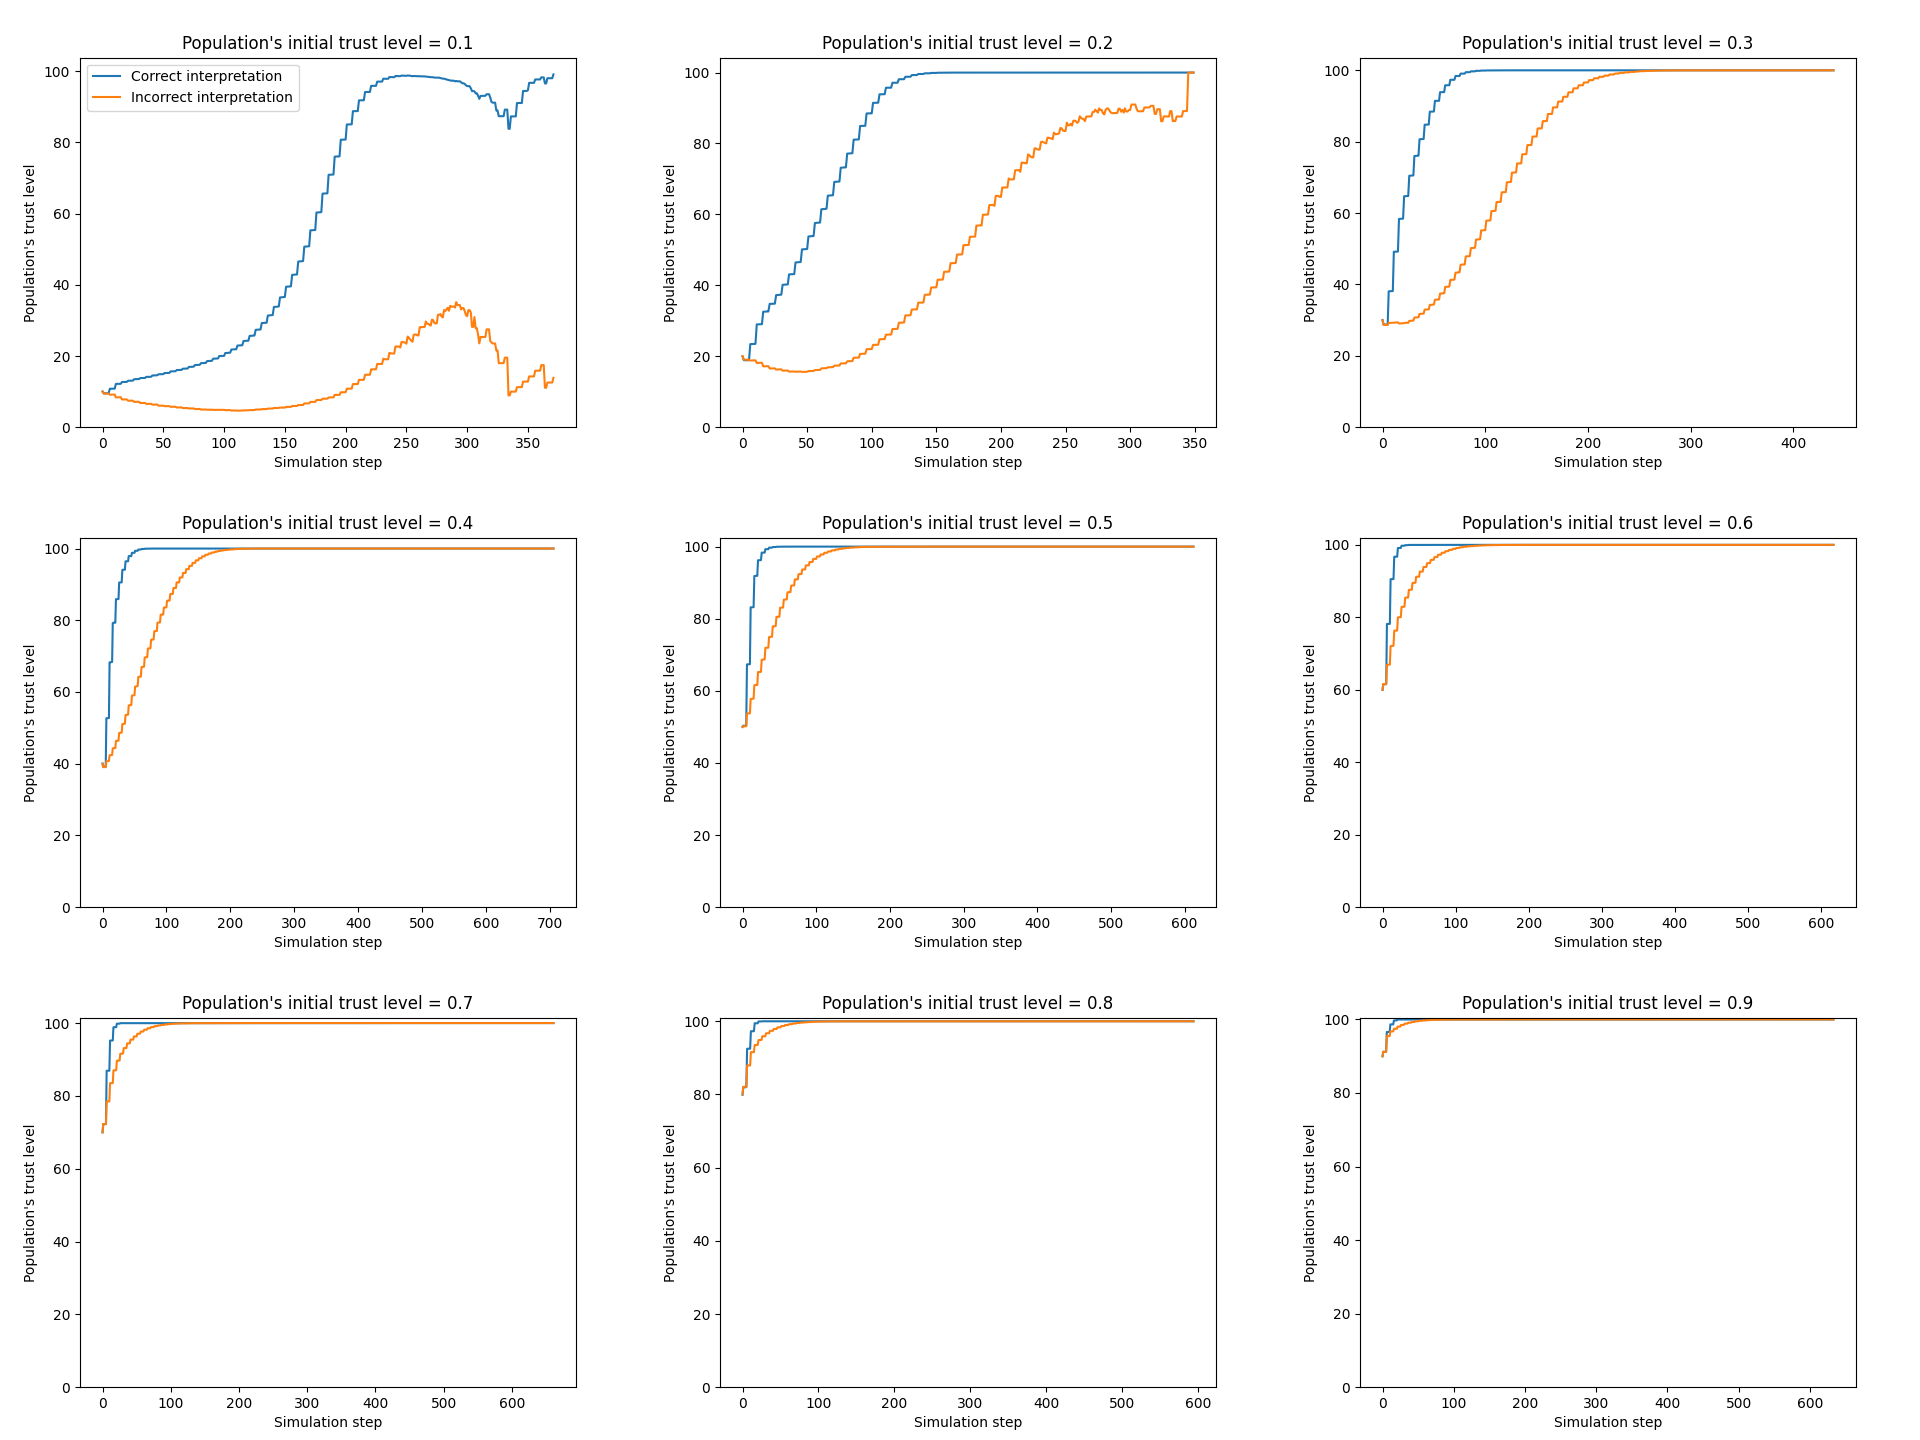
\includegraphics[width=\linewidth]{pics/TM.png}
    \endminipage{}
    \caption{Average population's trust level per misinterpretation status at each simulation step for each population's initial trust level. The number of simulation steps (x-axis) is different between graphs.}
    \label{fig:tm}
\end{figure}

\pagebreak

\subsection{Deceased, vaccinated and misinterpretation}

Figure \ref{fig:dvm} shows, with four curves, the evolution in time of the number of agents in the Deceased state per vaccination and misinterpretation statuses for each value of the population's trust level entry parameter. The first curve represents the number of agents which deceased being unvaccinated and interpreting the given information correctly. The second curve represents the number of agents which deceased being unvaccinated and interpreting the given information incorrectly. The third curve represents the number of agents which deceased being vaccinated and interpreting the given information correctly. Finally, the fourth curve represents the number of agents which deceased being vaccinated and interpreting the given information incorrectly. See figure \ref{fig:dvm_landscape} in appendix for a wider version.

From this figure, it is possible to see that:
\begin{enumerate}
    \item Reported agents with a Deceased state are mainly unvaccinated agents, as vaccinated agents are almost always reported to be 0. This is due to the choice to configure the model's vaccine as a highly effective vaccine (see section \ref{concept_vaccination_status}).
    \item There is a distinct gap between both unvaccinated groups of now deceased agents when the population's initial average trust is low, even average (from 0.1 to 0.5 included). This gap tends to shrink as the population's initial average trust gets higher. It is clear that unvaccinated agents misinterpreting information given to them have a higher death rate than those having a correct interpretation of the same information when the average trust of the population is low. In other words, a high population's initial average trust tends to negate the effect of misinterpretation.
\end{enumerate}

\begin{figure}[!htb]
    \centering
    \minipage{0.78\textwidth}
        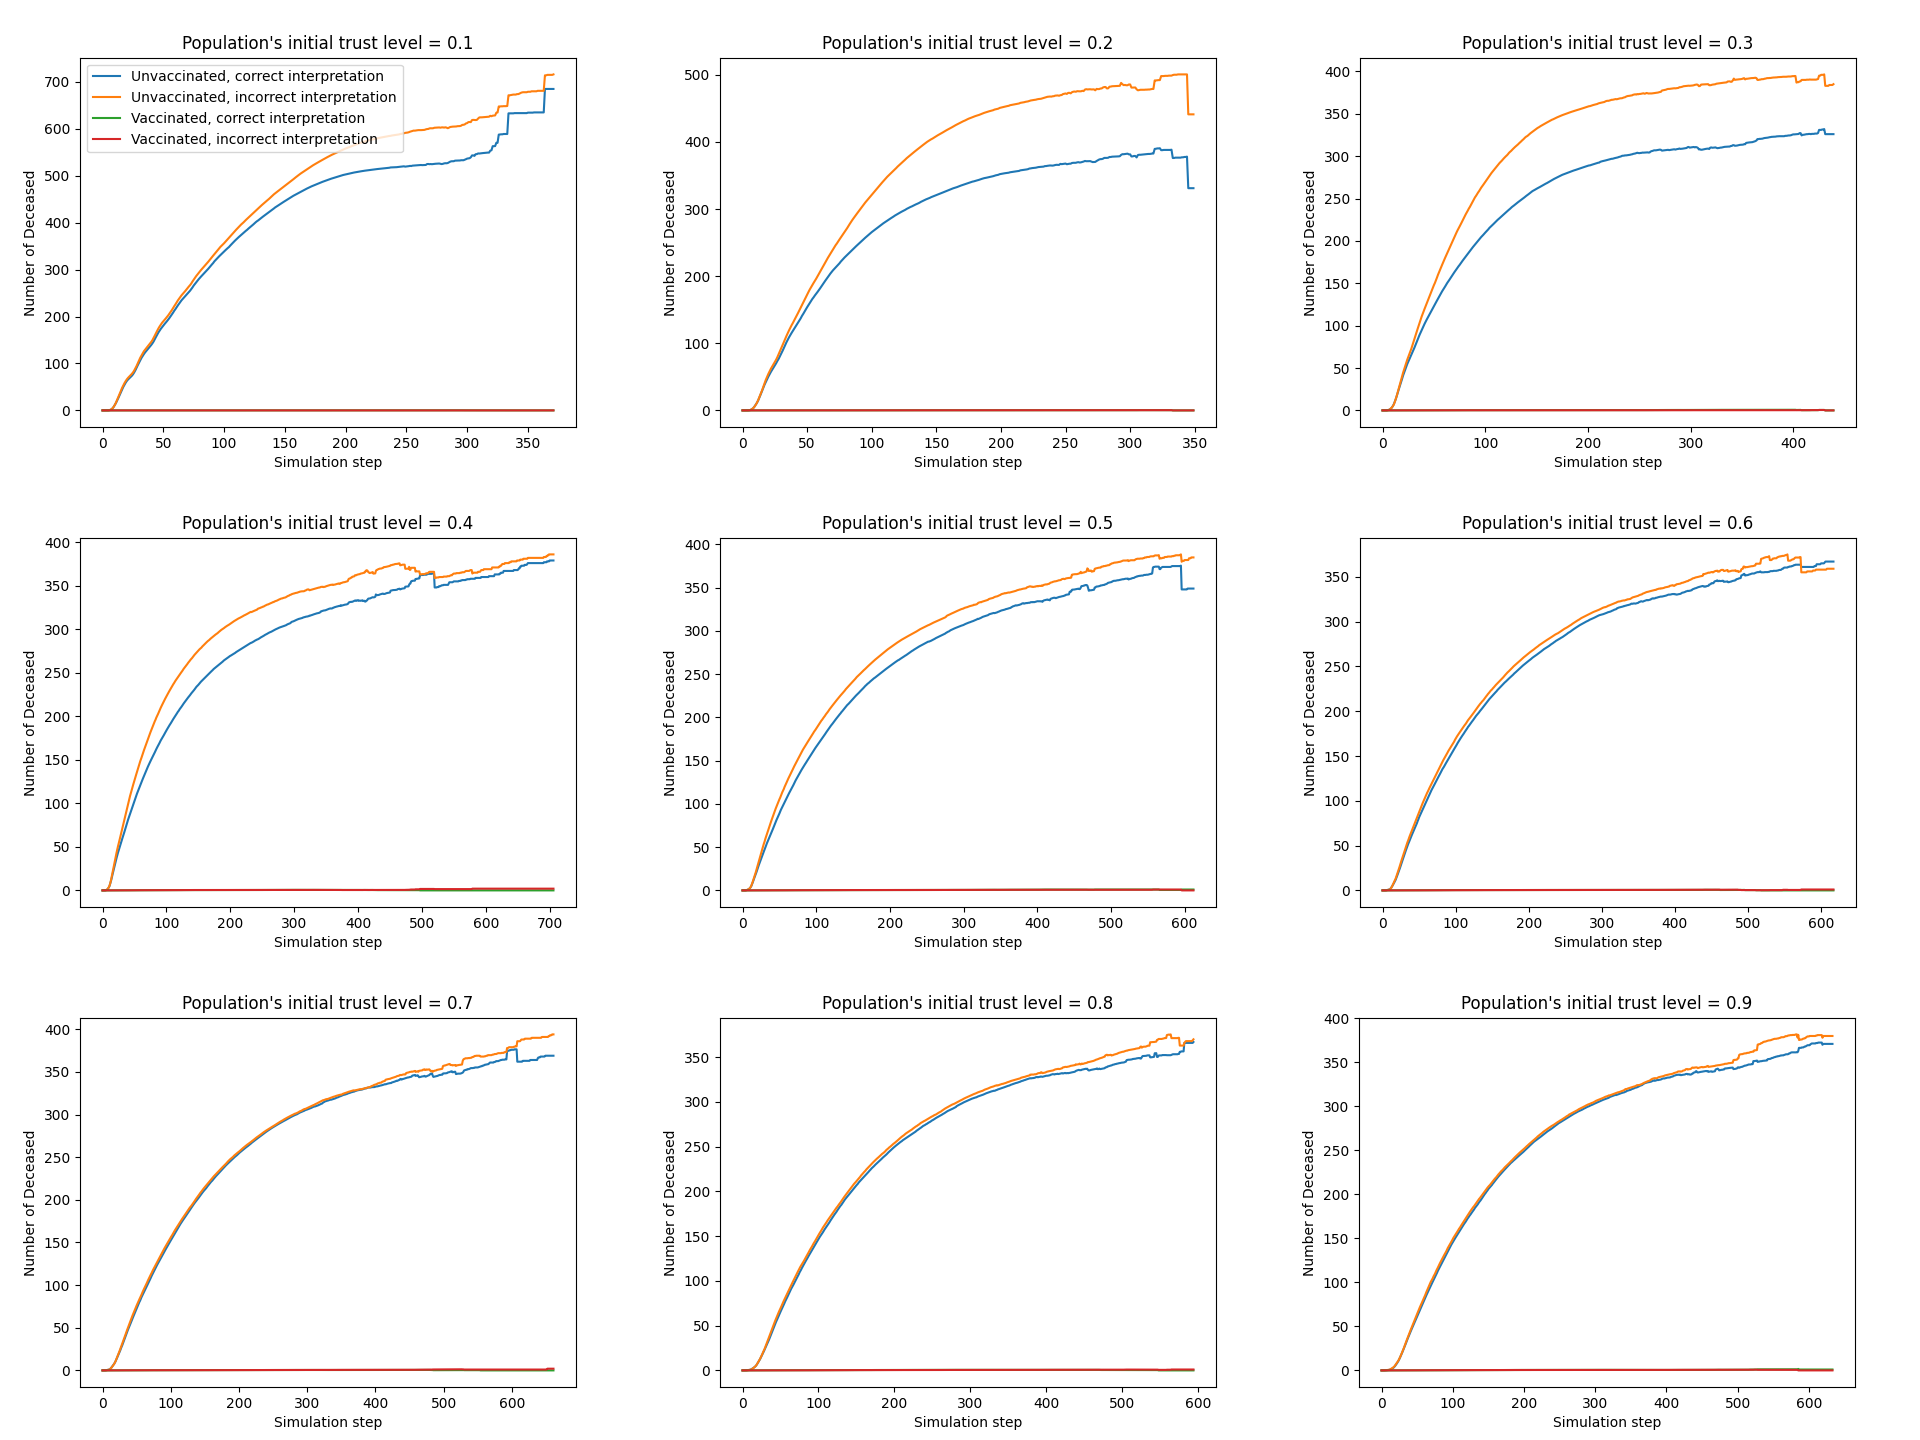
\includegraphics[width=\linewidth]{pics/DVM.png}
    \endminipage{}
    \caption{Average number of deaths per vaccination and misinterpretation statuses at each simulation step for each population's initial trust level. The number of simulation steps (x\babelhyphen{nobreak}axis) is different between graphs.}
    \label{fig:dvm}
\end{figure}
